\begin{figure*}
	\centering
	\begin{tikzpicture}[
	node distance = 1cm,
	%nodes=draw,
	auto,
	scale=1.0,
	transform shape,
	triangle/.style = {regular polygon, regular polygon sides=3 },
	node rotated/.style = {rotate=180},
	border rotated/.style = {shape border rotate=180}
	]
	
	%%%%%%%%%%%%%%%%%%%%%%%%%%%%%%%%%%%%%%%%%%%%%%%%%%%%%%%%%%%%%%%%%%%%%%%%%%%%
	% 4. Word hypotheses
	\node[ 
	line width=0.2mm,
	rounded corners=10pt, 
	%rectangle, draw, 
	minimum height=9cm, 
	minimum width=0.95\textwidth]
	at (0,0) 
	(word_hypotheses)
	{};
	
	\node[
	line width=0.2mm,
	rounded corners=2pt, 
	%rectangle, draw, 
	minimum height=0cm, 
	minimum width=0cm]
	at ([xshift=0em] word_hypotheses.north)
	(cosine)
	{
		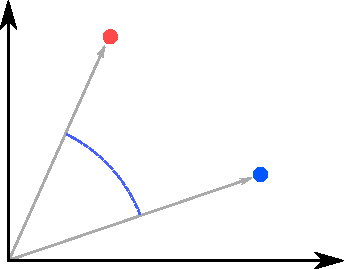
\includegraphics[width=3cm]{gfx/cosine}
	};
	\node at ([xshift=-2.6em, yshift=-1.9em] word_hypotheses.north) {$\alpha$};
	
	\node[
	line width=0.2mm,
	rounded corners=2pt, 
	%rectangle, draw, 
	minimum height=3cm, 
	minimum width=3cm]
	at ([yshift=1em, xshift=0em] cosine.north)
	(query_label)
	{
		\normalsize Cosine Similarity
	};
	
	
	\node[
	line width=0.2mm,
	rounded corners=2pt, 
	%rectangle, draw, 
	minimum height=3cm, 
	minimum width=3cm]
	at ([yshift=1em, xshift=8em] cosine.east)
	(query_captain)
	{
		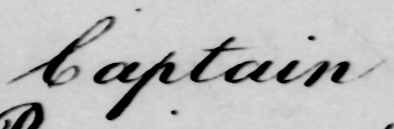
\includegraphics[width=3cm]{images/captain_query}
	};

	\node[
	line width=0.2mm,
	rounded corners=2pt, 
	%rectangle, draw, 
	minimum height=3cm, 
	minimum width=3cm]
	at ([yshift=-2em, xshift=0em] query_captain.north)
	(query_label)
	{
		\normalsize QUERY
	};
	%\node[anchor=south west,inner sep=0] (image) at (0,0) {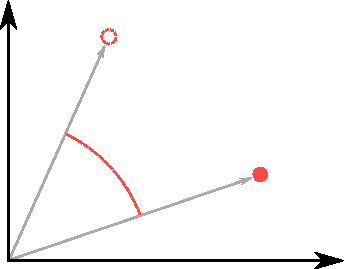
\includegraphics[width=0.28\textwidth]{gfx/cosine_embedding_problem}};
	
	% % % % % LENET % % % % % % %
	\node[ 
	rounded corners=3pt,
	%rectangle, draw,
	minimum height=3.4cm, 
	minimum width=4.5cm]
	at ([yshift=0em, xshift=1.75cm] word_hypotheses.west)
	(lenet)
	{
		%\Large{Architectures}
		%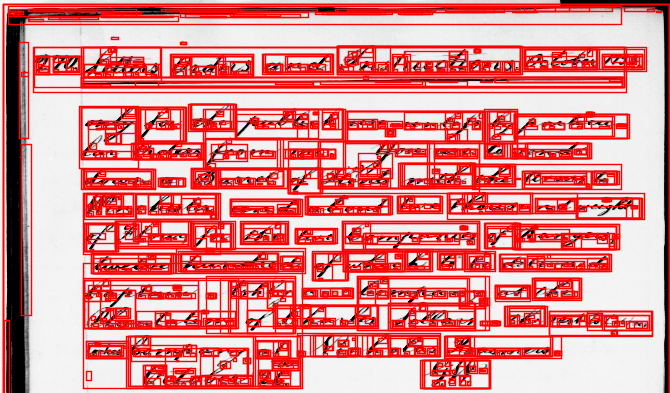
\includegraphics[width=5cm]{images/sift_regions_top.png}
	};
	\node[
	rounded corners=3pt,
	rectangle, draw,
	minimum height=0.0cm, 
	minimum width=4.2cm,
	fill=green!50]
	(conv1)
	at ([yshift=0.3cm, xshift=0.0cm] lenet.south)
	{
		\tiny{1 x Convolution}	
	};
	\node[
	rounded corners=3pt,
	rectangle, draw,
	minimum height=0.0cm, 
	minimum width=4.2cm,
	fill=orange!50]
	(pool1)
	at ([yshift=0.75em, xshift=0cm] conv1.north)
	{
		\tiny{Pooling}	
	};
	\node[
	rounded corners=3pt,
	rectangle, draw,
	minimum height=0.0cm, 
	minimum width=3.5cm,
	fill=green!50]
	(conv2)
	at ([yshift=0.75em, xshift=0cm] pool1.north)
	{
		\tiny{1 x Convolution}	
	};
	\node[
	rounded corners=3pt,
	rectangle, draw,
	minimum height=0.0cm, 
	minimum width=3.5cm,
	fill=cyan!50]
	(tpp)
	at ([yshift=0.75em, xshift=0cm] conv2.north)
	{
		\tiny{Temporal Pyramid Pooling}	
	};
	\node[
	rounded corners=3pt,
	rectangle, draw,
	minimum height=0.0cm, 
	minimum width=3.0cm,
	fill=magenta!50]
	(fc1)
	at ([yshift=0.75em, xshift=0cm] tpp.north)
	{
		\tiny{Fully Connected}	
	};
	\node[
	rounded corners=3pt,
	rectangle, draw,
	minimum height=0.0cm, 
	minimum width=3.0cm,
	fill=magenta!50]
	(fc2)
	at ([yshift=0.75em, xshift=0cm] fc1.north)
	{
		\tiny{Fully Connected}	
	};
	\node[
	rounded corners=3pt,
	rectangle, draw,
	minimum height=0.0cm, 
	minimum width=3.0cm,
	fill=yellow!50]
	(phoc_tpp)
	at ([yshift=0.75em, xshift=0cm] fc2.north)
	{
		\tiny{PHOC}	
	};
	% % % % % % % % % % % % % % % % % % % % % % % % % % % % % % % % %
	
	% % % % % TPP-PHOCNET % % % % % % % % % % % % % % % % % % % % % %
	\node[ 
	right = 0.0cm of lenet,
	rounded corners=3pt,
	%rectangle, draw,
	minimum height=4.7cm, 
	minimum width=4.5cm]
	%at (lenet.west)
	(tppnet)
	{
		%\Large{TPP-PHOCNet}
		%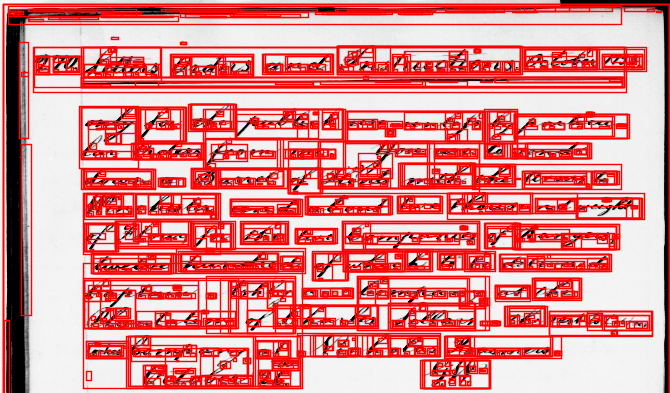
\includegraphics[width=5cm]{images/sift_regions_top.png}
	};
	\node[
	rounded corners=3pt,
	rectangle, draw,
	minimum height=0.0cm, 
	minimum width=4.2cm,
	fill=green!50]
	(conv1)
	at ([yshift=0.3cm, xshift=0cm] tppnet.south)
	{
		\tiny{2 x Convolution}	
	};
	\node[
	rounded corners=3pt,
	rectangle, draw,
	minimum height=0.0cm, 
	minimum width=4.2cm,
	fill=orange!50]
	(pool1)
	at ([yshift=0.75em, xshift=0cm] conv1.north)
	{
		\tiny{Pooling}	
	};
	\node[
	rounded corners=3pt,
	rectangle, draw,
	minimum height=0.0cm, 
	minimum width=3.5cm,
	fill=green!50]
	(conv2)
	at ([yshift=0.75em, xshift=0cm] pool1.north)
	{
		\tiny{2 x Convolution}	
	};
	\node[
	rounded corners=3pt,
	rectangle, draw,
	minimum height=0.0cm, 
	minimum width=3.5cm,
	fill=orange!50]
	(pool2)
	at ([yshift=0.75em, xshift=0cm] conv2.north)
	{
		\tiny{Pooling}	
	};
	\node[
	rounded corners=3pt,
	rectangle, draw,
	minimum height=0.0cm, 
	minimum width=3.0cm,
	fill=green!50]
	(conv3)
	at ([yshift=0.75em, xshift=0cm] pool2.north)
	{
		\tiny{6 x Convolution}	
	};
	\node[
	rounded corners=3pt,
	rectangle, draw,
	minimum height=0.0cm, 
	minimum width=3.0cm,
	fill=green!50]
	(conv4)
	at ([yshift=0.75em, xshift=0cm] conv3.north)
	{
		\tiny{3 x Convolution}	
	};
	\node[
	rounded corners=3pt,
	rectangle, draw,
	minimum height=0.0cm, 
	minimum width=3.0cm,
	fill=cyan!50]
	(tpp)
	at ([yshift=0.75em, xshift=0cm] conv4.north)
	{
		\tiny{Temporal Pyramid Pooling}	
	};
	\node[
	rounded corners=3pt,
	rectangle, draw,
	minimum height=0.0cm, 
	minimum width=3.0cm,
	fill=magenta!50]
	(fc1)
	at ([yshift=0.75em, xshift=0cm] tpp.north)
	{
		\tiny{Fully Connected}	
	};
	\node[
	rounded corners=3pt,
	rectangle, draw,
	minimum height=0.0cm, 
	minimum width=3.0cm,
	fill=magenta!50]
	(fc2)
	at ([yshift=0.75em, xshift=0cm] fc1.north)
	{
		\tiny{Fully Connected}	
	};
	\node[
	rounded corners=3pt,
	rectangle, draw,
	minimum height=0.0cm, 
	minimum width=3.0cm,
	fill=yellow!50]
	(phoc_tpp)
	at ([yshift=0.75em, xshift=0cm] fc2.north)
	{
		\tiny{PHOC}	
	};
	
	% % % % % % % % % % % % % % % % % % % % % % % % % % % % % % % % % %
	
	% % % % % RESNET % % % % % % %
	\node[ 
	right = 0.0cm of tppnet,
	rounded corners=3pt,
	%rectangle, draw,
	minimum height=5.5cm, 
	minimum width=4.5cm]
	%at (lenet.west)
	(resnet)
	{
		\Large{PHOCResNet}
		%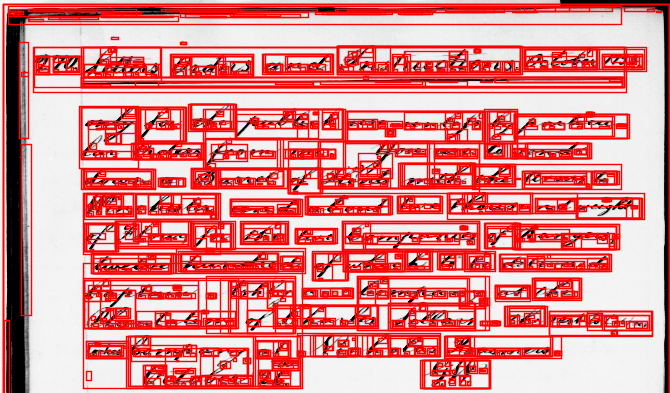
\includegraphics[width=5cm]{images/sift_regions_top.png}
	};
	\node[
	rounded corners=3pt,
	rectangle, draw,
	minimum height=0.0cm, 
	minimum width=4.2cm,
	fill=green!50]
	(conv1)
	at ([yshift=0.3cm, xshift=0.0cm] resnet.south)
	{
		\tiny{1 x Convolution}	
	};
	\node[
	rounded corners=3pt,
	rectangle, draw,
	minimum height=0.0cm, 
	minimum width=4.2cm,
	fill=orange!50]
	(pool1)
	at ([yshift=0.75em, xshift=0cm] conv1.north)
	{
		\tiny{Pooling}	
	};
	\node[
	rounded corners=3pt,
	rectangle, draw,
	minimum height=2.5cm, 
	minimum width=3.5cm,
	fill=black!10]
	(resnetblock)
	at ([yshift=3.8em, xshift=0cm] pool1.north)
	{
		%empty	
	};
	\node[
	rounded corners=3pt,
	rectangle, draw,
	minimum height=0.0cm, 
	minimum width=1.5cm,
	fill=green!50]
	(block_conv1)
	at ([yshift=1.85em, xshift=0cm] resnetblock.south)
	{
		\tiny{Convolution}	
	};
	\node[
	rounded corners=3pt,
	rectangle, draw,
	minimum height=0.0cm, 
	minimum width=1.5cm,
	fill=green!50]
	(block_conv2)
	at ([yshift=1.1em, xshift=0cm] block_conv1.north)
	{
		\tiny{Convolution}	
	};
	\node[
	rounded corners=3pt,
	rectangle, draw,
	minimum height=0.0cm, 
	minimum width=1.5cm,
	fill=green!50]
	(block_conv3)
	at ([yshift=1.1em, xshift=0cm] block_conv2.north)
	{
		\tiny{Convolution}	
	};
	
	\node[
	%rounded corners=3pt,
	%ellipse, draw,
	minimum height=-1.0cm, 
	minimum width=-1.0cm]
	(start)
	at ([yshift=-0.75em, xshift=0cm] block_conv1.south)
	{
			\Huge{.}
	};
	
	\node[
	%rounded corners=3pt,
	%ellipse, draw,
	minimum height=-1.0cm, 
	minimum width=-1.0cm]
	(end)
	at ([yshift=0.75em, xshift=0cm] block_conv3.north)
	{
			\Huge{.}
	};
	
	\node[
	rounded corners=3pt,
	rectangle, draw,
	minimum height=0.0cm, 
	minimum width=3.5cm,
	fill=cyan!50]
	(tpp_resnet)
	at ([yshift=0.75em, xshift=0cm] resnetblock.north)
	{
		\tiny{Temporal Pyramid Pooling}	
	};
	\node[
	rounded corners=3pt,
	rectangle, draw,
	minimum height=0.0cm, 
	minimum width=3.0cm,
	fill=magenta!50]
	(fc1)
	at ([yshift=0.75em, xshift=0cm] tpp_resnet.north)
	{
		\tiny{Fully Connected}	
	};
	\node[
	rounded corners=3pt,
	rectangle, draw,
	minimum height=0.0cm, 
	minimum width=3.0cm,
	fill=magenta!50]
	(fc2)
	at ([yshift=0.75em, xshift=0cm] fc1.north)
	{
		\tiny{Fully Connected}	
	};
	\node[
	rounded corners=3pt,
	rectangle, draw,
	minimum height=0.0cm, 
	minimum width=3.0cm,
	fill=yellow!50]
	(phoc_tpp)
	at ([yshift=0.75em, xshift=0cm] fc2.north)
	{
		\tiny{PHOC}	
	};
	
	
	\draw[line width=0.25mm, -stealth] (start) arc [x radius = 1.5cm, y radius = 1.03cm, start angle = -90,end angle = +90] (end);
	
	\draw[line width=0.27mm] (pool1) -- (block_conv1);
	
	\draw[line width=0.27mm] (block_conv1) -- (block_conv2);
	
	\draw[line width=0.27mm] (block_conv2) -- (block_conv3);
	
	\draw[line width=0.27mm] (block_conv3) -- (tpp_resnet);
	
	% % % % % % % % % % % % % % % % % % % % % % % % % % % % % % % % %

	
	% % % % % PHOCDenseNet % % % % % % %
	\node[ 
	right = 0.0cm of resnet,
	rounded corners=3pt,
	%rectangle, draw,
	minimum height=5.5cm, 
	minimum width=4.5cm]
	%at (lenet.west)
	(densenet)
	{
		%\Large{PHOCResNet}
		%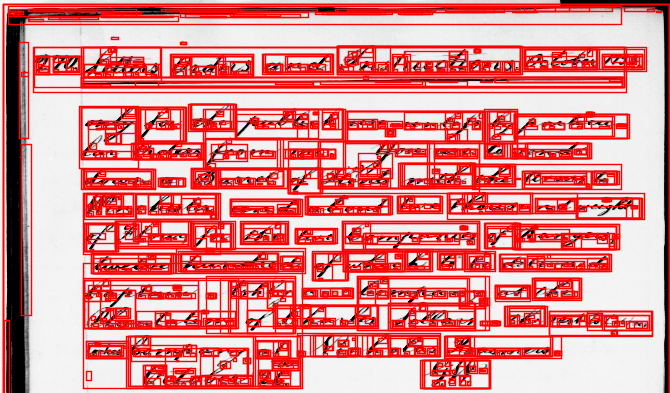
\includegraphics[width=5cm]{images/sift_regions_top.png}
	};
	\node[
	rounded corners=3pt,
	rectangle, draw,
	minimum height=0.0cm, 
	minimum width=4.2cm,
	fill=green!50]
	(dense_conv1)
	at ([yshift=0.3cm, xshift=0.0cm] densenet.south)
	{
		\tiny{1 x Convolution}	
	};
	\node[
	rounded corners=3pt,
	rectangle, draw,
	minimum height=0.0cm, 
	minimum width=4.2cm,
	fill=orange!50]
	(dense_pool1)
	at ([yshift=0.75em, xshift=0cm] dense_conv1.north)
	{
		\tiny{Pooling}	
	};
	\node[
	rounded corners=3pt,
	rectangle, draw,
	minimum height=2.5cm, 
	minimum width=3.5cm,
	fill=black!10]
	(denseblock)
	at ([yshift=3.8em, xshift=0cm] dense_pool1.north)
	{
		% frame for denseblock
		%\tiny{1xCONV [14,14,50]}	
	};
	\node[
	rounded corners=3pt,
	rectangle, draw,
	minimum height=0.0cm, 
	minimum width=1.5cm,
	fill=green!50]
	(denseblock_conv1)
	at ([yshift=1.35em, xshift=0cm] denseblock.south)
	{
		\tiny{Dense Block}	
	};
	\node[
	rounded corners=3pt,
	rectangle, draw,
	minimum height=0.0cm, 
	minimum width=1.5cm,
	fill=green!50]
	(denseblock_conv2)
	at ([yshift=1.5em, xshift=0cm] denseblock_conv1.north)
	{
		\tiny{Dense Block}	
	};
	\node[
	rounded corners=3pt,
	rectangle, draw,
	minimum height=0.0cm, 
	minimum width=1.5cm,
	fill=green!50]
	(denseblock_conv3)
	at ([yshift=1.5em, xshift=0cm] denseblock_conv2.north)
	{
		\tiny{Dense Block}	
	};
	
	\node[
	%rounded corners=3pt,
	%ellipse, draw,
	minimum height=-1.0cm, 
	minimum width=-1.0cm]
	(dense_start)
	at ([yshift=-0.5em, xshift=0cm] denseblock_conv1.south)
	{
		\Huge{.}
	};
	
	\node[
	%rounded corners=3pt,
	%ellipse, draw,
	minimum height=-1.0cm, 
	minimum width=-1.0cm]
	(dense_node_1)
	at ([yshift=0.5em, xshift=0cm] denseblock_conv1.north)
	{
		\Huge{.}
	};
	
	\node[
	%rounded corners=3pt,
	%ellipse, draw,
	minimum height=-1.0cm, 
	minimum width=-1.0cm]
	(dense_node_2)
	at ([yshift=0.5em, xshift=0cm] denseblock_conv2.north)
	{
		\Huge{.}
	};
	
	\node[
	%rounded corners=3pt,
	%ellipse, draw,
	minimum height=-1.0cm, 
	minimum width=-1.0cm]
	(dense_end)
	at ([yshift=0.6em, xshift=0cm] denseblock_conv3.north)
	{
		\Huge{.}
	};
	
	\node[
	rounded corners=3pt,
	rectangle, draw,
	minimum height=0.0cm, 
	minimum width=3.5cm,
	fill=cyan!50]
	(tpp_densenet)
	at ([yshift=0.75em, xshift=0cm] denseblock.north)
	{
		\tiny{Temporal Pyramid Pooling}	
	};
	\node[
	rounded corners=3pt,
	rectangle, draw,
	minimum height=0.0cm, 
	minimum width=3.0cm,
	fill=magenta!50]
	(dense_fc1)
	at ([yshift=0.75em, xshift=0cm] tpp_densenet.north)
	{
		\tiny{Fully Connected}	
	};
	\node[
	rounded corners=3pt,
	rectangle, draw,
	minimum height=0.0cm, 
	minimum width=3.0cm,
	fill=magenta!50]
	(dense_fc2)
	at ([yshift=0.75em, xshift=0cm] dense_fc1.north)
	{
		\tiny{Fully Connected}	
	};
	\node[
	rounded corners=3pt,
	rectangle, draw,
	minimum height=0.0cm, 
	minimum width=3.0cm,
	fill=yellow!50]
	(dense_phoc_tpp)
	at ([yshift=0.75em, xshift=0cm] dense_fc2.north)
	{
		\tiny{PHOC}	
	};
	
	
	\draw[line width=0.25mm, -stealth] (dense_start) arc [x radius = 1.5cm, y radius = 0.366cm, start angle = -90,end angle = +90] (dense_node_1);
	\draw[line width=0.25mm, -stealth] (dense_node_1) arc [x radius = 1.5cm, y radius = 0.366cm, start angle = -90,end angle = +90] (dense_node_2);
	\draw[line width=0.25mm, -stealth] (dense_node_2) arc [x radius = 1.5cm, y radius = 0.366cm, start angle = -90,end angle = +90] (dense_end);
	
	\draw[line width=0.25mm] (dense_start) arc [x radius = 1.5cm, y radius = 0.73cm, start angle = -90,end angle = +90] (dense_node_2);
	\draw[line width=0.25mm] (dense_node_1) arc [x radius = 1.5cm, y radius = 0.73cm, start angle = -90,end angle = +90] (dense_node_2);

	\draw[line width=0.25mm] (dense_start) arc [x radius = 1.5cm, y radius = 1.09cm, start angle = -90,end angle = +90] (dense_node_2);
		
	\draw[line width=0.27mm] (dense_pool1) -- (denseblock_conv1);
	
	\draw[line width=0.27mm] (denseblock_conv1) -- (denseblock_conv2);
	
	\draw[line width=0.27mm] (denseblock_conv2) -- (denseblock_conv3);
	
	\draw[line width=0.27mm] (denseblock_conv3) -- (tpp_densenet);
	
	% % % % % % % % % % % % % % % % % % % % % % % % % % % % % % % % %
	
	\node[ 
	%line width=0.1mm,
	rounded corners=3pt, 
	%rectangle, draw, 
	minimum height=1cm, 
	minimum width=1cm]
	at ([xshift=0em, yshift=1em] word_hypotheses.south)
	(captain)
	{
		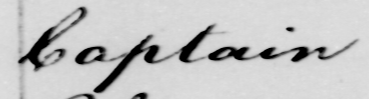
\includegraphics[width=3cm]{./images/captain.png}
	};


	\draw[line width=0.27mm, red, dashed, -stealth] (query_captain.west) -- ([yshift=2.5em, xshift=-5.8em] cosine.east);
	
	
	\draw[line width=0.27mm, -stealth] ([yshift=1em] captain.west) -- (lenet.south);
	
	\draw[line width=0.27mm, -stealth] ([xshift=-2em] captain.north) -- (tppnet.south);
	
	\draw[line width=0.27mm, -stealth] ([xshift=2em] captain.north) -- (resnet.south);
	
	\draw[line width=0.27mm, -stealth] ([yshift=1em] captain.east) -- (densenet.south);
	
	
	% lines from CNNs to cosine embedding
	
	\draw[line width=0.27mm, blue!100, dashed, -stealth] (lenet.north) -- ([yshift=-0.95em, xshift=-2.7em] cosine.east);
	
	\draw[line width=0.27mm, blue!100, dashed, -stealth] (tppnet.north) -- ([yshift=-1.2em, xshift=-2.65em] cosine.east);
	
	\draw[line width=0.27mm, blue!100, dashed, -stealth] (resnet.north) -- ([yshift=-1.2em, xshift=-2.3em] cosine.east);
	
	\draw[line width=0.27mm, blue!100, dashed, -stealth] (densenet.north) -- ([yshift=-1.1em, xshift=-2.0em] cosine.east);
		
	%%%%%%%%%%%%%%%%%%%%%%%%%%%%%%%%%%%%%%%%%%%%%%%%%%%%%%%%%%%%%%%%%%%%%%%%%%%%
	
	\end{tikzpicture}
	\caption{Overview of the explored CNN architectures. The networks are from left to right, PHOCLeNet, TPP-PHOCNet, PHOCResNet, and PHOCDenseNet. The CNNs are trained to predict a desired word string embedding generated from the annotation. Word spotting can then be performed in the embedding space through a simple nearest neighbor search using the cosine similarity as distance metric. Please note, that due to space issues this overview is not an exactly architecture description especially for the residual bottleneck and dense blocks. 
	The exactly description is given in Sec. \ref{sec:method}.}
	\label{fig:architectures_overview}
\end{figure*}
